% !TeX spellcheck = en_US
\chapter{Overview}
This if my learning notes for \ac{RL}. \ac{RL} are approaches for learning decision making from experience. In the \ac{AI} context, many \ac{RL} algorithms handle the scarcity of available (human-annotated) data.

\begin{displayquote}
	\textit{Instead of trying to produce a program to simulate the adult mind, why not rather try to produce one which simulates the child's? If this were then subjected to an appropriate course of education, one would obtain the adult brain.} - Alan Turing -
\end{displayquote}

A \ac{RL} problem has 3 major blocks as follows:
\begin{figure}[hbt!]
	\centering
	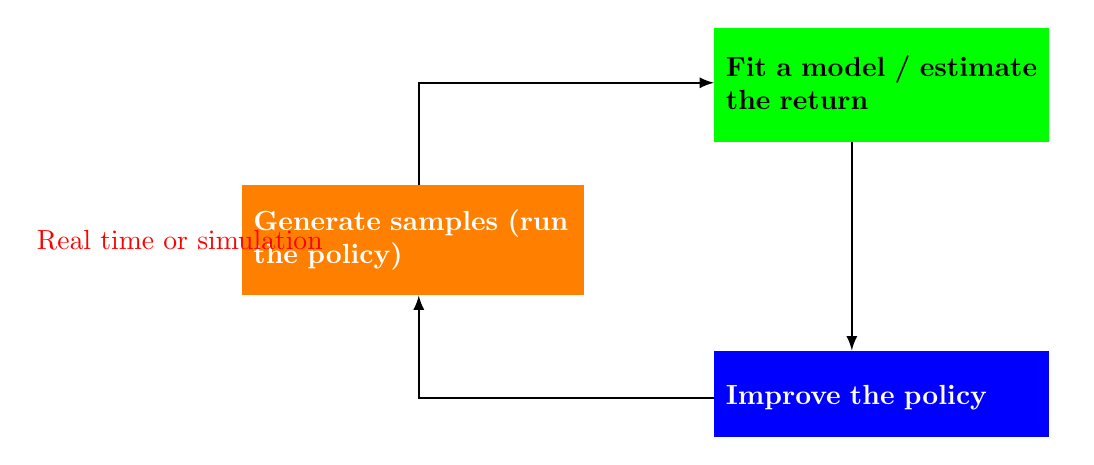
\begin{tikzpicture}
		\fill[green, very thick] (.25,1.25) rectangle (4.5,2.7);
		\fill[blue, very thick] (.25,-1.4) rectangle (4.5,-2.5);
		\fill[orange, very thick] (-5.75,-.7) rectangle (-1.4,.7);
		\node[black, text width=4.2cm] at (2.5,2) {\textbf{Fit a model / estimate the return}};
		\node[white, text width=4.2cm] at (2.5,-2) {\textbf{Improve the policy}};
		\node[white, text width=4.2cm] at (-3.5,0) {\textbf{Generate samples (\ie run the policy)}};
		\node[red, text width=3.7cm] at (-6.5,0) {Real time or simulation};
		\draw[thick, -latex] (2,1.25) -- (2,-1.4);
		\draw[thick, -latex] (.25,-2) -- (-3.5,-2) -- (-3.5,-.7);
		\draw[thick, -latex] (-3.5,.7) -- (-3.5,2) -- (.25,2);
	\end{tikzpicture}
	\caption{Structure of \ac{RL} algorithms.}
	\label{fig:RL-structure}
\end{figure}

\section{Learning resources}
\begin{itemize}
	\item \href{http://rail.eecs.berkeley.edu/deeprlcourse/}{Deep \ac{RL} - CS285, UC Berkeley - Sergey Levine}
	\item \href{http://ai.berkeley.edu/lecture_videos.fhtml}{CS188 Berkeley AI}
	\item The book \textit{Reinforcement learning: An introduction} \cite{sutton2018reinforcement}
	\item \href{https://www.tensorflow.org/agents/overview}{\texttt{TensorFlow} Agents' tutorial}
	\item \href{https://simoninithomas.github.io/Deep_reinforcement_learning_Course/#}{A Free course in Deep RL}
\end{itemize}

\section{Terminology \& Notation}
\begin{itemize}
	\item Check out \ac{MDP} and \ac{POMDP} in the \href{robotics.pdf}{robotic notes} or the \ac{RL} book by \citeaus{sutton2018reinforcement}.
	\item $\textbf{s}_t$ - state
	\item $\textbf{o}_t$ - observation
	\item $\textbf{a}_t$ - action
	\item $\pi_{\theta}(\textbf{a}_t | \textbf{o}_t)$ - policy (or $\pi_{\theta}(\textbf{a}_t | \textbf{s}_t)$ for fully observed scenario)
	\item $r(\textbf{s}_t, \textbf{a}_t)$ - reward or $c(\textbf{s}_t, \textbf{a}_t)$ - cost
	\item $\tau$ - trajectory (as sequence of states and actions)
	\[ p_\theta(\tau) = p_\theta(\textbf{s}_1, \textbf{a}_1, \dots, \textbf{s}_T, \textbf{a}_T) = p(\textbf{s}_1) \prod_{t=1}^{T} \pi_\theta(\textbf{a}_t | \textbf{s}_t) p(\textbf{s}_{t+1} | \textbf{s}_t, \textbf{a}_t) \]
	\item The Q-function is the expectation of total reward, from the q-state $(\textbf{s}_t, \textbf{a}_t)$, under policy $\pi_\theta$.
	\begin{equation}
		Q^\pi (\textbf{s}_t, \textbf{a}_t) = \sum_{t' = t}^{T} \mathbb{E}_{\pi_\theta} \left[ r(\textbf{s}_{t'}, \textbf{a}_{t'}) | \textbf{s}_t, \textbf{a}_t \right]
	\end{equation}
	\item The value function is the expectation of total reward, from the state $\textbf{s}_t$, under policy $\pi_\theta$.
	\begin{equation}
		V^\pi (\textbf{s}_t) = \sum_{t' = t}^{T} \mathbb{E}_{\pi_\theta} \left[ r(\textbf{s}_{t'}, \textbf{a}_{t'}) | \textbf{s}_t \right] = \mathbb{E}_{\textbf{a}_t \sim \pi(\textbf{a}_t | \textbf{s}_t)} Q^\pi (\textbf{s}_t, \textbf{a}_t)
	\end{equation}
\end{itemize}

\begin{figure}[hbt!]
	\centering
	\begin{tikzpicture}[
		roundnode/.style={circle, draw=black!60, very thick, minimum size=7mm}]
		\node[roundnode](o1){$\textbf{o}_1$};
		\node[roundnode](a1)[right=of o1]{$\textbf{a}_1$};
		\node[roundnode](o2)[right=of a1]{$\textbf{o}_2$};
		\node[roundnode](a2)[right=of o2]{$\textbf{a}_2$};
		\node[roundnode](o3)[right=of a2]{$\textbf{o}_3$};
		\node[roundnode](a3)[right=of o3]{$\textbf{a}_3$};		
		\node[roundnode](s1)[below left=of a1]{$\textbf{s}_1$};
		\node[roundnode](s2)[below left=of a2]{$\textbf{s}_2$};	
		\node[roundnode](s3)[below left=of a3]{$\textbf{s}_3$};
		\draw[-latex](o1.east) -- (a1.west) node[midway, above]{$\pi_{\theta}$};
		\draw[-latex](o2.east) -- (a2.west) node[midway, above]{$\pi_{\theta}$};
		\draw[-latex](o3.east) -- (a3.west) node[midway, above]{$\pi_{\theta}$};
		\draw[-latex](s1.east) -- (s2.west) node[midway, below]{$p(\textbf{s}_{t+1} | \textbf{s}_t, \textbf{a}_t)$};
		\draw[-latex](s2.east) -- (s3.west) node[midway, below]{$p(\textbf{s}_{t+1} | \textbf{s}_t, \textbf{a}_t)$};
		\draw[-latex](s1.north) -- (o1.south);
		\draw[-latex](s2.north) -- (o2.south);
		\draw[-latex](s3.north) -- (o3.south);
		\draw[-latex](a1.south east) -- (s2.north west);
		\draw[-latex](a2.south east) -- (s3.north west);
	\end{tikzpicture}
	\caption{The relationship between state $\textbf{s}_t$, observation $\textbf{o}_t$ and action $\textbf{a}_t$.}
\end{figure}

\section{Overview on RL Algorithms}
\ac{RL} problem revolves around maximizing the expectation of total rewards. We aim to find the \ac{param} to maximize the expected value of the sum of rewards, under the trajectory distribution.
\begin{equation}
	\theta^* = \underset{\theta}{\arg\max}\; \mathbb{E}_{\tau \sim p_\theta(\tau)} \left[ \sum_t r(\textbf{s}_t, \textbf{a}_t) \right]
\end{equation}

There are many methods / algorithms with their trade-offs and assumptions:
\begin{itemize}
	\item Sampling efficiency \& stability and ease of use
	\item Stochastic or deterministic
	\item Continuous or discrete
	\item Episode or infinite horizon
\end{itemize}
\tabref{tab:RL-algors} gives an overview and comparison between algorithms.

\section{Current State of the Art}
Some current \ac{SOTA} \ac{RL} \ac{algor}s are:
\begin{itemize}
	\item \ac{DQN}: model-free \ac{RL} for discrete action spaces \cite{mnih2015human}
	\item \ac{DDPG}: model-free \ac{RL} for continuous action spaces \cite{lillicrap2015continuous}
\end{itemize}

\section{Challenges}
\begin{itemize}
	\item Humans can learn incredibly quickly
	\item Humans can reuse past knowledge\\
	Transfer learning in Deep \ac{RL} is an open problem
	\item Not clear what the reward function should be
	\item Not clear what the role of prediction should be
\end{itemize}

\begin{landscape}
	\begin{table}[htb!]
		\centering
		\begin{tblr}{colspec={X[0.6]||X|X[1.1]|X[0.8]|X}, row{1} = {l}}
			& Model-based & Value function fitting & Actor-critic & Policy Gradient \\ \hline\hline
			\textbf{\textit{Sample efficiency}} \newline {\fontsize{8}{0}\selectfont (How many samples do we need to get good policy?)}
			& \SetCell[c=4]{l}{\newline 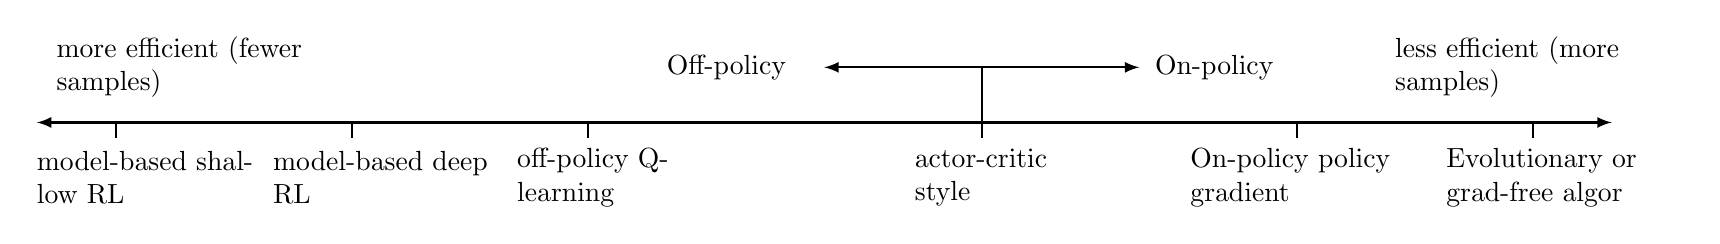
\begin{tikzpicture}[baseline=0]
					\draw[thick,latex-latex] (-10,0) -- (10,0);
					\draw[thick] (-9,0) -- (-9,-0.2);
					\node[text width=3cm] at (-8.5,-.7) {model-based shallow \ac{RL}};
					\draw[thick] (-6,0) -- (-6,-0.2);
					\node[text width=3cm] at (-5.5,-.7) {model-based deep \ac{RL}};
					\draw[thick] (2,0.7) -- (2,0);
					\draw[thick, latex-latex] (0,0.7) -- (4,0.7);
					\draw[thick] (-3,0) -- (-3,-.2);
					\node[text width=3cm] at (-2.4,-.7) {off-policy Q-learning};
					\draw[thick] (2,0) -- (2,-.2);
					\node[text width=2.5cm] at (2.4,-.7) {actor-critic style};
					\draw[thick] (6,0) -- (6,-.2);
					\node[text width=2.7cm] at (6,-.7) {On-policy policy gradient};
					\draw[thick] (9,0) -- (9,-.2);
					\node[text width=3cm] at (9.4,-.7) {Evolutionary or grad-free \ac{algor}};
					\node[text width=4cm] at (0,0.7) {Off-policy};
					\node[text width=4cm] at (6.2,0.7) {On-policy};
					\node[text width=3.5cm] at (-8,.7) {\hlr{more efficient (fewer samples)}};
					\node[text width=3.5cm] at (9,.7) {\hlr{less efficient (more samples)}};
				\end{tikzpicture} \newline\newline - Sometimes, with simulated experiences, we can use \hlr{less efficient} \ac{algor} \newline \hlr{Wall clock time $\neq$ efficiency} \newline - More assumptions, as we go to the left } \\ \hline	
			\SetCell[r=2]{l}{\textbf{\textit{Stability \& ease of use}} \newline {\fontsize{9}{0}\selectfont - Does it converge? \newline - If yes, to what? \newline - Does it \hlr{always} converge?}} & \SetCell[c=4]{l}{\hlr{\ac{RL} is often not \ac{GD}}} \\
			& Model will converge.\newline \hlb{BUT}, better model do \hlr{NOT GUARANTEE} better policy &
			Minimize error of fit \newline At worst case, doesn't optimize anything.\newline Un-provable convergence \newline \hlr{$\Rightarrow$ more like heuristics} & &
			\hlr{is \ac{GD}}\newline least efficient + assumptions \\ \hline				
			\textbf{\textit{Assumption}} &
			By some: episode learning &
			\hlb{Generally}: \newline full observability. \newline By some continuous method: continuity / smoothness & &
			By pure policy gradient methods: \newline \hlb{Often:} episode learning \\ \hline				
			\textbf{\textit{Example}} & 
			- Dyna \newline - Guided policy search &
			- Q-learning \newline - DQN \newline - Temporal difference \newline - Fitted value iteration &
			- \ac{A3C} \cite{mnih2016icml} \newline - \ac{SAC} \cite{haarnoja2018soft} &
			- REINFORCE \cite{williams1992jml} \newline - Natural policy gradient \cite{kakade2001natural} \newline - Trusted Region policy optimization \cite{schulman2015icml}
		\end{tblr}
		\caption{Different \ac{RL} algorithms.}
		\label{tab:RL-algors}
	\end{table}
\end{landscape}
